\ifx\XeTeXversion\undefined\pdfoutput=1\fi
\documentclass[11pt,reqno]{amsart}

\usepackage[margin=1in]{geometry}
\usepackage{amsmath,amssymb,amsthm,mathtools}
\usepackage{booktabs,array,multirow}
\usepackage{graphicx}
\usepackage{xcolor}
\usepackage{enumitem}
\usepackage{microtype}
\usepackage{listings}
% Allow line breaks after underscores inside long Lean identifiers
\let\origunderscore\_
\renewcommand{\_}{\origunderscore\allowbreak}
\setlength{\emergencystretch}{3em}
\usepackage[colorlinks=true,linkcolor=blue!60!black,citecolor=teal!70!black,urlcolor=blue!70!black]{hyperref}
\pdfstringdefDisableCommands{\let\_\origunderscore}

% Theorem environments
\newtheorem{theorem}{Theorem}[section]
\newtheorem{proposition}[theorem]{Proposition}
\newtheorem{lemma}[theorem]{Lemma}
\newtheorem{corollary}[theorem]{Corollary}
\theoremstyle{definition}
\newtheorem{definition}[theorem]{Definition}
\newtheorem{remark}[theorem]{Remark}

% Clean code listings (pure ASCII safe for arXiv pdflatex)
\lstdefinelanguage{Lean4}{
  keywords={abbrev,def,noncomputable,theorem,lemma,structure,inductive,where,if,then,else,fun,by,in,forall,exists,Set,Fin,Real,Matrix,Equiv,Perm},
  sensitive=true,
  morecomment=[l]{--},
  morecomment=[s]{/-}{-/}
}
\lstset{
  language=Lean4,
  basicstyle=\ttfamily\footnotesize,
  keywordstyle=\bfseries\color{blue!60!black},
  commentstyle=\itshape\color{black!55},
  frame=single,
  framerule=0.4pt,
  rulecolor=\color{black!25},
  backgroundcolor=\color{black!2},
  xleftmargin=0.8em,
  xrightmargin=0.8em,
  aboveskip=0.8em,
  belowskip=0.8em,
  breaklines=true,
  columns=fullflexible
}

% Standard notation
\newcommand{\R}{\mathbb{R}}
\newcommand{\C}{\mathbb{C}}
\newcommand{\Q}{\mathbb{Q}}
\newcommand{\Z}{\mathbb{Z}}
\newcommand{\N}{\mathbb{N}}
\newcommand{\Sph}{\mathbb{S}^2}
\newcommand{\ip}[2]{\langle #1, #2 \rangle}
\newcommand{\norm}[1]{\lVert #1 \rVert}
\newcommand{\Frob}[1]{\lVert #1 \rVert_{\mathrm{F}}}
\newcommand{\TTP}{X_{\mathrm{TTP}}}
\newcommand{\Ettphi}{E_{\mathrm{ttp,hi}}}

\title[The Thomson Problem for Nine Points on the Sphere]{%
The Tricapped Trigonal Prism Is the Unique Minimizer of the Coulomb Energy of Nine Points on the Sphere}

\author{Yang Li}
\address{Changsha University of Science and Technology, Changsha, China}
\email{ly3069777195@outlook.com}

\subjclass[2020]{Primary 52A40, 31C20; Secondary 90C22, 68V20, 52C17}
\keywords{Thomson problem, Coulomb energy, spherical codes, three-point semidefinite programming bounds, tricapped trigonal prism, computer-assisted proof, Lean~4}

\date{November 23, 2026}

\begin{document}

\begin{abstract}
We prove that among all configurations of nine distinct points on the unit sphere $\Sph \subset \R^3$, the Coulomb energy
\[
  E(x) = \sum_{1 \le i < j \le 9} \frac{1}{\norm{x_i - x_j}}
\]
is globally minimized by the $D_{3h}$ tricapped trigonal prism $\TTP(z^*)$ with optimal prism half-height $z^* \approx 0.70364839580413177578$ and minimum energy $E(\TTP(z^*)) \approx 25.75998653126983156408$, and that every global minimizer is obtained from $\TTP(z^*)$ by an orthogonal transformation of $\R^3$ and a relabeling of the points.

Our computer-assisted proof splits into just two cases at the minimum pairwise inner product $m = \min_{i<j}\ip{x_i}{x_j} = -9/10$.
For $m \le -9/10$, a single $(2,7)$-typed degree-$10$ three-point semidefinite certificate ($M=6$, $K=6$) strictly excludes all configurations by a margin exceeding $5.5 \times 10^{-3}$.
For $m \ge -9/10$, an $S_3$-equivariant degree-$18$ three-point semidefinite certificate ($M=10$, $K=10$), which incorporates higher azimuthal harmonics beyond $K = 6$, gives a certified lower bound within $1.2 \times 10^{-17}$ of $E(\TTP(z^*))$ (and within $1.48 \times 10^{-16}$ of our rational upper bound $\Ettphi$); combined with a $7$-piece degree-$37$ Bernstein polynomial certificate, it confines every pairwise inner product of any low-energy configuration within $10^{-4}$ of the six inner-product levels of $\TTP(z^*)$.
An exact interval-arithmetic $3$- and $4$-point Gram determinant screen together with a $28$-leaf symmetry-broken depth-first proof tree establishes combinatorial rigidity to the $S_9$ orbit of $\TTP(z^*)$, a quantitative Procrustes bound places the aligned configuration in a Frobenius ball of radius $1/500$, and a rotational gauge-fixing, Bregman--Young, and $27\times 27$ integer-Cholesky Hessian analysis proves strict local minimality with quadratic coercivity constant $1/30$.

Every algebraic identity, positive semidefiniteness claim, polynomial nonnegativity certificate, combinatorial search, and analytic estimate is formally verified inside the Lean~4 kernel over Mathlib (Lean~\texttt{v4.34.1}) using exact integer and rational arithmetic---employing binary bit-tries and $19$ parallel two-dimensional Kronecker evaluation slices---with zero \texttt{sorry}s, no \texttt{native\_decide}, and only Lean's three standard axioms (\texttt{propext}, \texttt{Classical.choice}, \texttt{Quot.sound}).
\end{abstract}

\maketitle

\section{Introduction}\label{sec:intro}

Given $N$ distinct points $x = (x_1,\dots,x_N)$ on the unit sphere $\Sph = \{v \in \R^3 : \norm{v} = 1\}$, the classical \emph{Thomson problem}~\cite{Thomson1904} asks for the global minimizers of the discrete Coulomb energy
\begin{equation}\label{eq:energy}
  E(x) \;=\; \sum_{1 \le i < j \le N} \frac{1}{\norm{x_i - x_j}} \;=\; \sum_{1 \le i < j \le N} \varphi(\ip{x_i}{x_j}),
  \qquad \varphi(t) := \frac{1}{\sqrt{2 - 2t}}.
\end{equation}
Although global minima have been investigated numerically for over a century~\cite{ErberHockney1991,WalesUlker2006}, rigorous proofs of global optimality and uniqueness remain exceptionally scarce.
For $N \in \{2, 3, 4, 6, 12\}$, global optimality holds universally across all completely monotonic potentials of squared distance, following classical linear programming bounds~\cite{Yudin1992,Andreev1996,KolushovYudin1997} and the universal-optimality framework of Cohn and Kumar~\cite{CohnKumar2007}.
The five-point case $N = 5$ was resolved by Schwartz~\cite{Schwartz2013,Schwartz2023} via a computer-assisted branch-and-bound proof showing that the triangular bipyramid is the unique minimizer.
More recently, three-point semidefinite programming bounds~\cite{BachocVallentin2008,CohnWoo2012} combined with exact computer verification settled the cases $N = 8$, where Kryvonos, Liehr, and Taylor~\cite{KLT2026} proved global optimality and uniqueness of the square antiprism with a Lean~4 verification (see also the Lean~4 development of Tooby-Smith and Zughaid~\cite{TZ2026}), and $N = 7$, where a Lean~4 proof established that the regular pentagonal bipyramid is the unique minimizer~\cite{ValsN72026}.

In this paper we settle the nine-point Thomson problem, proving both global optimality and rigid $O(3) \times S_9$ uniqueness of the $D_{3h}$ tricapped trigonal prism (TTP), and providing a complete kernel-checked formalization in Lean~4.

\subsection{Why $N = 9$ presents new obstacles---and how they collapse}\label{subsec:obstacles}
Compared with $N = 7$ and $N = 8$, the nine-point problem introduces three interacting difficulties:
\begin{enumerate}[leftmargin=2.2em]
  \item \emph{No antipodal pair and non-transitive two-orbit geometry.} Unlike the pentagonal bipyramid ($N=7$, which has antipodal poles at $t=-1$) and the vertex-transitive square antiprism ($N=8$, single vertex orbit), the $D_{3h}$ tricapped trigonal prism has \emph{two} vertex orbits (six prism vertices at heights $\pm z^*$ and three equatorial caps at height $0$), no antipodal pair ($\min_{i<j}\ip{x_i}{x_j} \approx -0.74756$), and six distinct pairwise inner-product levels $\nu_0(z^*) < \dots < \nu_5(z^*)$ with multiplicities $(6,6,3,3,6,12)$.
  \item \emph{Higher azimuthal harmonics.} Write $(M,K)$ for a three-point SDP hierarchy with $K$ azimuthal harmonic orders $0 \le k < K$ (blocks $F_0,\dots,F_{K-1}$) and polynomial block size $M-k$. In our numerical experiments, truncating at $K = 6$ ($0 \le k \le 5$) left an energy gap of order $10^{-4}$ for every $M \le 10$. With $K = M$ the gap fell from $4.12 \times 10^{-4}$ at $(8,8)$ to $4.70 \times 10^{-5}$ at $(9,9)$ and $9.96 \times 10^{-20}$ at $(10,10)$; in the $(10,10)$ solution the harmonic blocks $F_6, F_7$ are active while $F_8, F_9$ are numerically negligible ($\sim 10^{-28}$).
  \item \emph{Equivariant reduction and two-certificate simplicity.} Exploiting full $S_3$ permutation symmetry of triples on the cap $m \ge -9/10$ decomposes the SOS Gram matrices into one-dimensional trivial/sign blocks and a single two-dimensional standard irreducible block, shrinking the semidefinite problem dramatically and eliminating all intermediate strip subdivisions. Remarkably, the entire sphere $[-1,1]$ is covered by \emph{just two} three-point SDP certificates:
  \begin{itemize}[leftmargin=1.5em]
    \item a single $(2,7)$-typed slab certificate at $(M,K)=(6,6)$ strictly excluding $m \le -9/10$ by margin $> 5.54 \times 10^{-3}$; and
    \item a single $S_3$-invariant cap certificate at $(M,K)=(10,10)$ on $m \ge -9/10$ whose integer Cholesky form is certified to within $1.2 \times 10^{-17}$ of $E(\TTP(z^*))$ ($1.48 \times 10^{-16}$ below $\Ettphi$).
  \end{itemize}
\end{enumerate}

\subsection{Main theorem}\label{subsec:main-thm}
For cylindrical coordinates $\mathrm{cyl}(\rho,\theta,h) := (\rho\cos\theta, \rho\sin\theta, h) \in \R^3$ and any $z \in (0,1)$, define the nine-point $D_{3h}$ tricapped trigonal prism $\TTP(z) : \{0,\dots,8\} \to \Sph$ (indexing vertices $0,\dots,8$ henceforth to match Lean's \texttt{Fin 9}) by
\begin{equation}\label{eq:ttp-def}
  \TTP(z)_i := \begin{cases}
    \mathrm{cyl}\!\left(\sqrt{1-z^2},\, \frac{2\pi i}{3},\, z\right), & i \in \{0,1,2\}, \\[4pt]
    \mathrm{cyl}\!\left(\sqrt{1-z^2},\, \frac{2\pi(i-3)}{3},\, -z\right), & i \in \{3,4,5\}, \\[4pt]
    \mathrm{cyl}\!\left(1,\, \frac{\pi}{3} + \frac{2\pi(i-6)}{3},\, 0\right), & i \in \{6,7,8\}.
  \end{cases}
\end{equation}

\begin{theorem}[Global optimality and uniqueness for $N=9$]\label{thm:main}
There exists $z^*$ with $\frac{d}{dz}E(\TTP(z))\big|_{z=z^*} = 0$ and
\begin{equation}\label{eq:zstar-interval}
  \begin{aligned}
  z^* &\in \left[\frac{28145935832165271}{40000000000000000},\; \frac{10994506184439559}{15625000000000000}\right] \\
      &= [0.703648395804131775,\; 0.703648395804131776]
  \end{aligned}
\end{equation}
such that:
\begin{enumerate}[label=\textup{(\roman*)},leftmargin=2.2em]
  \item For every configuration $x = (x_0,\dots,x_8)$ of nine distinct points on $\Sph$,
  \[
    E(\TTP(z^*)) \;\le\; E(x).
  \]
  \item Equality $E(x) = E(\TTP(z^*))$ holds if and only if there exist a linear isometry $g \in O(3)$ and a permutation $\sigma \in S_9$ such that $x_i = g(\TTP(z^*)_{\sigma(i)})$ for all $i \in \{0,\dots,8\}$.
\end{enumerate}
\end{theorem}

\begin{remark}[What exactly is formalized]\label{rem:formal-scope}
In the fixed challenge specification (Listing~\ref{lst:lean-stmt}), \texttt{thomson\_nine} asserts $\exists\,z \in (0,1)$ minimizing $E$, while \texttt{thomson\_nine\_unique} places $\exists\,z \in (0,1)$ inside $\forall\,x$ (so each global minimizer belongs to the $O(3)\times S_9$ orbit of $\TTP(z)$ for some $z$, without fixing a single $z$ across minimizers or stating the $\Leftarrow$ direction). In our Lean proof both theorems use the same witness $z^*$ from \texttt{LocalMinL6.exists\_z\_star} lying in~\eqref{eq:zstar-interval} with $\mathrm{critGap}(z^*) = 0$, and \texttt{Solution.lean} additionally exports the strengthened theorem \texttt{ThomsonN9.thomson\_nine\_main} (lines 764--816) with $\exists\,z^* \in [z^*_{\mathrm{lo}}, z^*_{\mathrm{hi}}]$ on the outside proving $\mathrm{critGap}(z^*) = 0$ and both parts~(i)--(ii) (including $\iff$) of Theorem~\ref{thm:main} verbatim. Lean proves only the rational upper bound $E(\TTP(z^*)) \le \Ettphi$ in~\eqref{eq:E-ttp-hi}; the $40$-digit value of $E(\TTP(z^*))$ comes from Section~\ref{subsec:stage-a}. Numerically $z^*$ is the unique stationary point of $z \mapsto E(\TTP(z))$ on $(0,1)$, which the proof does not need.
\end{remark}

\subsection{Formal verification summary}\label{subsec:formal-summary}
Theorem~\ref{thm:main} (both via the fixed challenge theorems and verbatim via \texttt{thomson\_nine\_main}; see Remark~\ref{rem:formal-scope}) is formally proved in Lean~4~\cite{deMouraUllrich2021} against Mathlib~\cite{Mathlib2020} (pinned toolchain \texttt{leanprover/lean4:v4.34.1}, Mathlib commit \texttt{d13f23b7}) in \texttt{formal/lean/ThomsonN9/Solution.lean} ($818$ lines). Its dependency cone within the project consists of $45$ modules ($20{,}327$ lines): the $32$ modules of \texttt{ThomsonN9/StageB/} written for this proof ($12{,}880$ lines, $1.75\,\mathrm{MB}$), \texttt{Solution.lean}, and $12$ earlier project modules (\texttt{TableB5*}, \texttt{TableB1*}, \texttt{TableA}, \texttt{M1Data}) supplying the Procrustes chain and the M1 bound.
All four challenge theorems fixed verbatim in \texttt{ComparatorChallenges/ThomsonN9.lean}---two warm-up lower bounds (\texttt{thomson\_nine\_M0}: $E \ge 18$; \texttt{thomson\_nine\_M1}: $E \ge 189/8$) together with \texttt{thomson\_nine} and \texttt{thomson\_nine\_unique}---as well as \texttt{thomson\_nine\_main} are proved with zero \texttt{sorry}s, zero soundness-affecting forbidden tokens, exact $36/36$ declaration matching under \texttt{pp.all} + \texttt{pp.universes}, and dependence solely on Lean's three standard axioms \texttt{propext}, \texttt{Classical.choice}, and \texttt{Quot.sound}.
In particular, \texttt{native\_decide} is never used; every certificate identity and search tree is checked inside the Lean kernel via \texttt{decide +kernel} ($57$ kernel-decision sites in the dependency cone). The supporting modules raise \texttt{maxHeartbeats} and \texttt{maxRecDepth}, which are resource limits only and do not affect soundness; \texttt{Solution.lean} itself contains no \texttt{set\_option}.

\section{Formal Statement and Geometry of the Tricapped Trigonal Prism}\label{sec:statement}

\subsection{Lean~4 formalization of the challenge statements}\label{subsec:lean-stmt}
The fixed specification file \texttt{ComparatorChallenges/ThomsonN9.lean} (unmodified since repository creation) defines the Euclidean space \texttt{R3}, admissible configurations \texttt{SphereConfig 9}, Coulomb energy \texttt{coulombEnergy}, cylindrical coordinates \texttt{cyl}, and the $D_{3h}$ family \texttt{triCapPrism}, and states four challenge theorems.
Listing~\ref{lst:lean-stmt} gives the definitions and the two main theorem statements from \texttt{ThomsonN9/Solution.lean} (lines 86--106, 696--698, and 722--725), transliterated to ASCII (e.g.\ \texttt{R} for $\R$, \texttt{||v||} for the norm, \texttt{equiv\_li} for linear isometric equivalence), with the proofs omitted.

\begin{lstlisting}[float=htbp,caption={Formal definitions and main theorems in \texttt{ThomsonN9/Solution.lean} (ASCII transliteration; checked verbatim against \texttt{ComparatorChallenges/\allowbreak ThomsonN9.lean}).},label={lst:lean-stmt}]
abbrev R3 := EuclideanSpace R (Fin 3)

def SphereConfig (n : Nat) : Set (Fin n -> R3) :=
  {x | (forall i, ||x i|| = 1) /\ Function.Injective x}

noncomputable def coulombEnergy {n : Nat} (x : Fin n -> R3) : R :=
  sum i : Fin n, sum j in Finset.Ioi i, ||x i - x j||^(-1)

noncomputable def cyl (rho theta h : R) : R3 :=
  ![rho * cos theta, rho * sin theta, h]

noncomputable def triCapPrism (z : R) : Fin 9 -> R3 := fun i =>
  if (i : Nat) < 3 then cyl (sqrt (1 - z ^ 2)) (2 * pi * (i : Nat) / 3) z
  else if (i : Nat) < 6 then cyl (sqrt (1 - z ^ 2)) (2 * pi * ((i : Nat) - 3) / 3) (-z)
  else cyl 1 (pi / 3 + 2 * pi * ((i : Nat) - 6) / 3) 0

theorem thomson_nine :
    exists z in Set.Ioo (0 : R) 1,
      forall x in SphereConfig 9,
        coulombEnergy (triCapPrism z) <= coulombEnergy x

theorem thomson_nine_unique :
    forall x in SphereConfig 9,
      (forall y in SphereConfig 9, coulombEnergy x <= coulombEnergy y) ->
        exists (g : R3 equiv_li R3) (sigma : Equiv.Perm (Fin 9))
               (z : R) (hz : z in Set.Ioo (0 : R) 1),
          forall i, x i = g (triCapPrism z (sigma i))
\end{lstlisting}

Three conventions are worth noting:
(i) \emph{Injectivity} (\texttt{Function.Injective x}) is essential because $0^{-1} = 0$ in Lean;
(ii) \emph{Uniqueness} is stated up to the full orthogonal group $O(3)$ ($\R^3 \simeq_{\mathrm{li}} \R^3$, including reflections; note $\TTP(z)$ is achiral since horizontal reflection swaps top and bottom triangles) and relabeling $\sigma \in S_9$;
(iii) \texttt{Solution.lean} also contains kernel-checked proofs of \texttt{thomson\_nine\_M0} ($E \ge 36/2 = 18$) and \texttt{thomson\_nine\_M1} ($E \ge 189/8 = 23.625$, via a degree-$8$ two-point LP certificate in \texttt{M1Data.lean}).

\subsection{Inner-product spectrum and stationarity of $\TTP(z)$}\label{subsec:ttp-geom}
Let $\rho(z) := \sqrt{1 - z^2}$ for $z \in (0,1)$. Direct evaluation of~\eqref{eq:ttp-def} shows that the $\binom{9}{2} = 36$ pairwise inner products of $\TTP(z)$ fall into exactly six curves $\nu_0(z),\dots,\nu_5(z)$, listed in Table~\ref{tab:ttp-spectrum} and illustrated in Figure~\ref{fig:ttp}.

\begin{figure}[htbp]
  \centering
  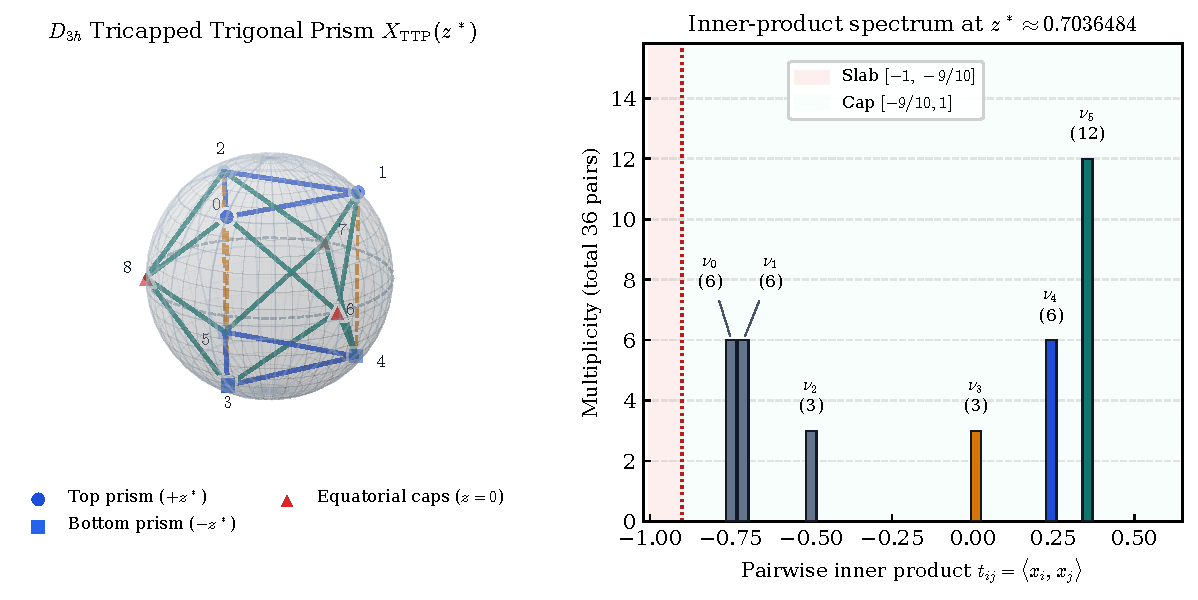
\includegraphics[width=0.96\textwidth]{figures/fig_ttp.pdf}
  \caption{Left: the $D_{3h}$ tricapped trigonal prism $\TTP(z^*)$ on $\Sph$ showing the top triangle ($0,1,2$), bottom triangle ($3,4,5$), equatorial caps ($6,7,8$), and the three shortest edge classes ($\nu_5$ teal, $\nu_4$ blue, $\nu_3$ dashed amber). Right: the inner-product spectrum across the $36$ pairs, showing the clean separation from the slab cut $t = -9/10$.}
  \label{fig:ttp}
\end{figure}

\begin{table}[htbp]
  \centering
  \caption{The six pairwise inner-product curves $\nu_k(z)$ of $\TTP(z)$, their multiplicities $m_k$ (summing to $36$), squared chordal distances $d_k^2 = 2 - 2\nu_k(z)$, and numerical values at the stationary point $z^* \approx 0.70364839580413177578$.}
  \label{tab:ttp-spectrum}
  \small
  \renewcommand{\arraystretch}{1.18}
  \setlength{\tabcolsep}{4pt}
  \begin{tabular}{@{}clccrr@{}}
    \toprule
    Index $k$ & Pair class & Mult.\ $m_k$ & Closed form $\nu_k(z)$ & $\nu_k(z^*)$ & Distance $d_k(z^*)$ \\
    \midrule
    $0$ & Top--bottom opposite & $6$ & $-\frac{1}{2}(1-z^2) - z^2 = -\frac{1+z^2}{2}$ & $-0.7475605325$ & $1.8695242884$ \\
    $1$ & Cap--prism opposite  & $6$ & $-\sqrt{1-z^2}$ & $-0.7105483341$ & $1.8496206822$ \\
    $2$ & Cap--cap             & $3$ & $-1/2$ & $-0.5000000000$ & $1.7320508076$ \\
    $3$ & Top--bottom vertical & $3$ & $1 - 2z^2$ & $0.0097578702$ & $1.4072967916$ \\
    $4$ & Top--top / bot--bot  & $6$ & $1 - \frac{3}{2}(1-z^2) = \frac{3z^2-1}{2}$ & $0.2426815974$ & $1.2307058159$ \\
    $5$ & Cap--prism adjacent  & $12$ & $\frac{1}{2}\sqrt{1-z^2}$ & $0.3552741670$ & $1.1355402529$ \\
    \bottomrule
  \end{tabular}
\end{table}

Summing $\varphi(\nu_k(z)) = (2 - 2\nu_k(z))^{-1/2}$ with multiplicities $m_k$ yields the closed-form family energy (\texttt{LocalMinL6.coulombEnergy9\_ttpPt}):
\begin{equation}\label{eq:E-family}
  E(\TTP(z)) \;=\; \frac{6}{\sqrt{3+z^2}} + \frac{6}{\sqrt{2+2\rho}} + \sqrt{3} + \frac{3}{2z} + \frac{6}{\sqrt{3}\,\rho} + \frac{12}{\sqrt{2-\rho}},
  \qquad \rho = \sqrt{1-z^2}.
\end{equation}
Differentiating~\eqref{eq:E-family} with respect to $z$ and removing the positive factor $6z$ gives the stationary gap function $\mathrm{critGap}(z) := \frac{1}{6z}\frac{d}{dz}E(\TTP(z))$ (\texttt{LocalMinL6.critGap}):
\begin{equation}\label{eq:crit-gap}
  \mathrm{critGap}(z)
  \;=\; \frac{3}{(\sqrt{3}\,\rho)^3} - \frac{2}{(2z)^3} - \frac{1}{(\sqrt{3+z^2})^3} - \frac{1}{\rho(\sqrt{2-\rho})^3} + \frac{1}{\rho(\sqrt{2+2\rho})^3}.
\end{equation}
On the $10^{-18}$-wide rational interval $[z^*_{\mathrm{lo}}, z^*_{\mathrm{hi}}]$ of~\eqref{eq:zstar-interval}, certified rational arithmetic verifies $\mathrm{critGap}(z^*_{\mathrm{lo}}) < 0 < \mathrm{critGap}(z^*_{\mathrm{hi}})$. By the Intermediate Value Theorem (\texttt{LocalMinL6.exists\_z\_star}), there exists $z^* \in [z^*_{\mathrm{lo}}, z^*_{\mathrm{hi}}] \subset (0,1)$ with $\mathrm{critGap}(z^*) = 0$, and $20$-digit rational square-root envelopes prove the strict rational upper bound
\begin{equation}\label{eq:E-ttp-hi}
  E(\TTP(z^*)) \;\le\; \Ettphi := \frac{257599865312698317}{10^{16}} \;=\; 25.7599865312698317.
\end{equation}
(The $50$-digit interval arithmetic of our independent Stage~A verification gives
\[
  \begin{aligned}
  E(\TTP(z^*)) \in [&\,25.759986531269831564075702273760494028636, \\
                    &\,25.759986531269831564075702273760494028648],
  \end{aligned}
\]
so $\Ettphi$ exceeds $E(\TTP(z^*))$ by $1.36 \times 10^{-16}$.)

\section{Overview of the Proof Architecture}\label{sec:overview}

Let $x \in \mathrm{SphereConfig}\;9$ be any nine-point unit-sphere configuration.
If $E(x) > \Ettphi$, then $E(\TTP(z^*)) \le \Ettphi < E(x)$ holds immediately by~\eqref{eq:E-ttp-hi}, and $x$ cannot be a global minimizer.
Assume therefore that $E(x) \le \Ettphi$, and let $m(x) := \min_{i < j} \ip{x_i}{x_j} \in [-1, 1)$.
The proof branches into two exhaustive cases at the rational threshold $-9/10$ (Figure~\ref{fig:overview}):

\begin{figure}[htbp]
  \centering
  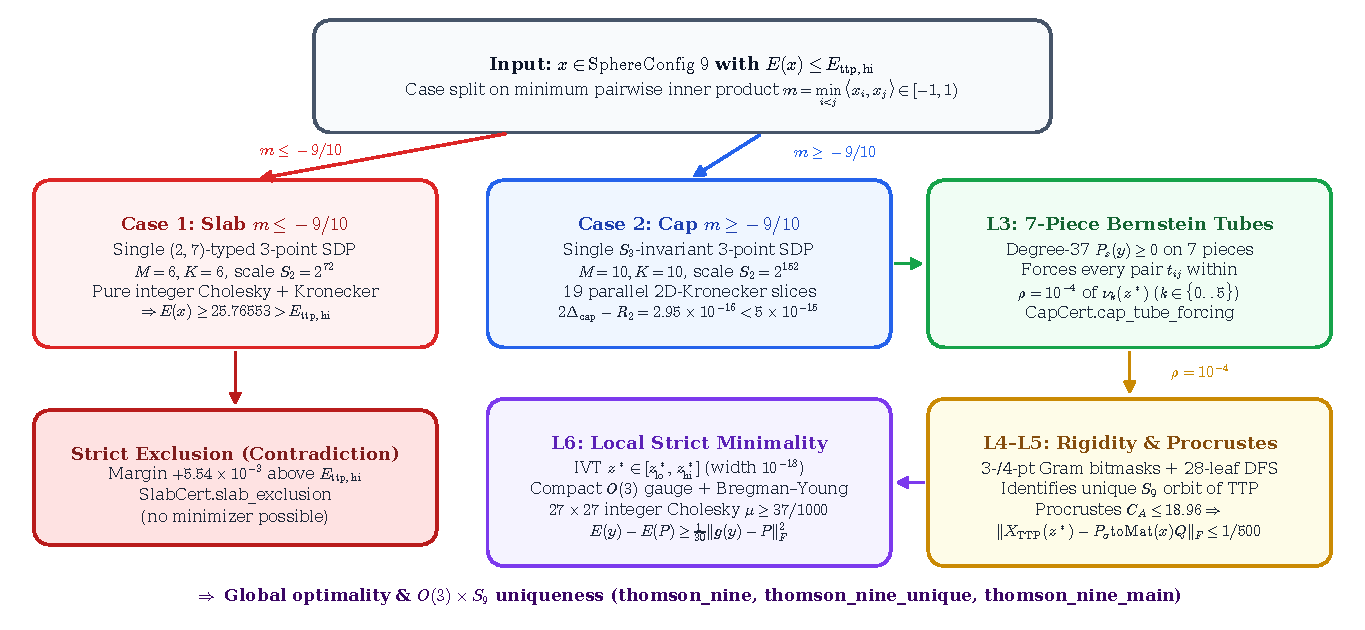
\includegraphics[width=0.98\textwidth]{figures/fig_overview.pdf}
  \caption{End-to-end architecture of the Thomson $N=9$ proof. Every arrow corresponds to a kernel-checked Lean~4 theorem in \texttt{ThomsonN9/StageB/}, assembled in \texttt{ThomsonN9/Solution.lean}.}
  \label{fig:overview}
\end{figure}

\begin{enumerate}[leftmargin=2.2em]
  \item \textbf{Case~1 (Slab $m(x) \le -9/10$, Section~\ref{sec:slab}):} Relabel so that $\ip{x_0}{x_1} \le -9/10$. Partitioning the vertices into two poles $\{0,1\}$ and seven ring points $\{2,\dots,8\}$, a single $(2,7)$-typed degree-$10$ three-point SDP certificate ($M=6$, $K=6$, scale $S_2 = 2^{72}$) proves
  \[
    E(x) \;\ge\; 25.76553265\ldots \;>\; \Ettphi,
  \]
  contradicting $E(x) \le \Ettphi$ with a margin exceeding $5.54 \times 10^{-3}$ (\texttt{SlabCert.slab\_exclusion}).
  \item \textbf{Case~2 (Cap $m(x) \ge -9/10$, Sections~\ref{sec:cap}--\ref{sec:local}):} All $36$ pairwise inner products lie in $[-9/10, 1)$. The argument proceeds in three quantitative steps:
  \begin{enumerate}[label=\textup{(\alph*)},leftmargin=1.8em]
    \item \emph{Sharp $S_3$-invariant cap certificate \& Bernstein tube forcing (Section~\ref{sec:cap}).} A single $S_3$-invariant degree-$18$ three-point SDP certificate ($M=10$, $K=10$, scale $S_2 = 2^{152}$) yields a minorant $H(t) \le (1+R_2)\varphi(t)$ and lower bound $e_{\mathrm{cap}} - 36 R_1 \le \sum_{i<j} H(t_{ij})$ with per-pair deficit budget $2\Delta_{\mathrm{cap}} - R_2 = 2.952 \times 10^{-16} < \varepsilon_y = 5 \times 10^{-15}$. A $7$-piece degree-$37$ Bernstein polynomial certificate on $y = \sqrt{(1-t)/2}$ excludes every value outside six narrow windows, forcing every pair $t_{ij}$ within $\rho = 10^{-4}$ of some $\nu_k(z^*)$ (\texttt{CapCert.cap\_tube\_forcing}).
    \item \emph{Combinatorial rigidity \& Procrustes ball entry (Section~\ref{sec:rigidity}).} Since $10^{-4} < g_{\min}/2 \approx 0.0185$, each pair acquires a unique color $c(i,j) \in \{0,\dots,5\}$. Certified interval arithmetic on $3\times 3$ and $4\times 4$ Gram determinants builds exact bitmasks of realizable triangles and $K_4$ subgraphs, and a symmetry-broken depth-first search certifies that every valid $9$-vertex coloring belongs to $28$ explicit leaves, each accompanied by an explicit permutation $\sigma \in S_9$ aligning it to the TTP pattern. Applying the quantitative Gram-to-coordinate Procrustes theorem (\texttt{TableB5Chain.chain\_convert\_A}, constant $C_A \le 18.957127$) yields $Q \in O(3)$ with $\Frob{\TTP(z^*) - P_\sigma \mathrm{toMat}(x) Q} \le C_A \cdot 10^{-4} < 1/500$ (\texttt{RigidityL4.rigidity\_to\_ball}).
    \item \emph{Local strict minimality \& uniqueness (Section~\ref{sec:local}).} Passing to $y_i = g_1(x_{\sigma(i)})$ via the linear isometry $g_1$ induced by $Q$, we have $\sum_{i=0}^8 \norm{y_i - \TTP(z^*)_i}^2 \le (1/500)^2$. Compact $O(3)$ maximization aligns $y$ into the symmetric Procrustes rotational gauge without increasing the chordal distance. Using exact criticality at $z^*$, a purely algebraic Bregman--Young quadratic lower bound on $\varphi$, and a $27\times 27$ integer-Cholesky lower bound $\mu_{\mathrm{pen}} \ge 37/1000$ on the penalized Hessian, we prove
    \[
      E(y) - E(\TTP(z^*)) \;\ge\; \frac{1}{30} \sum_{i=0}^8 \norm{g(y_i) - \TTP(z^*)_i}^2
    \]
    (\texttt{LocalMinL6.local\_min\_ball}), yielding both $E(\TTP(z^*)) \le E(x)$ and $O(3)\times S_9$ uniqueness.
  \end{enumerate}
\end{enumerate}

\section{Three-Point Positivity on $\Sph$ and Equivariant SDP Reductions}\label{sec:threepoint}

The sole geometric input to both SDP certificates is the three-point positive semidefiniteness theorem of Bachoc and Vallentin~\cite{BachocVallentin2008}, adapted to energy minimization by Cohn and Woo~\cite{CohnWoo2012}.

\subsection{Spherical three-point kernels}\label{subsec:kernels}
Define polynomials $Q_k(u,v,t)$ recursively (\texttt{StageB.Q3} in \texttt{ThreePoint.lean}) by
\begin{equation}\label{eq:Q3-rec}
  Q_0(u,v,t) = 1, \qquad Q_1(u,v,t) = t - uv, \qquad Q_{k+2} = 2(t-uv)Q_{k+1} - (1-u^2)(1-v^2)Q_k.
\end{equation}
For each harmonic order $k \ge 0$ and matrix size $m \ge 1$, let $Y_k(u,v,t)$ denote the $m \times m$ matrix with entries $(Y_k)_{ab}(u,v,t) = u^a v^b Q_k(u,v,t)$ ($0 \le a, b < m$).
In our Lean certificates, every PSD harmonic matrix $F_k \succeq 0$ is stored directly in exact integer Cholesky factorized form $F_k = \sum_{r} c_{k,r} c_{k,r}^\top$ with integer column vectors $c_{k,r} \in \Z^m$ (eliminating any remainder matrix $\Delta$); the corresponding scalar kernel is
\[
  \mathrm{harmBlkEv}_k(u,v,t) \;=\; Q_k(u,v,t) \sum_r p_{k,r}(u)\, p_{k,r}(v), \qquad p_{k,r}(u) := \sum_{a=0}^{m-1} (c_{k,r})_a u^a.
\]

\begin{lemma}[Three-point positivity on $\Sph$, \texttt{PolyKron.sum\_harmListEv\_nonneg}]\label{lem:3pt-pos}
Let $x_1,\dots,x_n \in \Sph$ be unit vectors with Gram entries $t_{ij} = \ip{x_i}{x_j}$, let $S \subseteq \{1,\dots,n\}$ be any subset of root indices, and let $h(u,v,t) = \sum_{k=0}^{K-1} \mathrm{harmBlkEv}_k(u,v,t)$ be a sum of Cholesky-factored harmonic blocks. Then
\[
  \sum_{i \in S} \sum_{j=1}^n \sum_{l=1}^n h(t_{ij}, t_{il}, t_{jl}) \;\ge\; 0.
\]
\end{lemma}

\begin{proof}
Fix a root $i \in S$ and decompose each $x_j$ orthogonally as $x_j = u_j x_i + w_j$ with $u_j = \ip{x_i}{x_j}$ and $w_j \perp x_i$, so $\norm{w_j}^2 = 1 - u_j^2$. Identifying $x_i^\perp$ isometrically with $\C$ sends $w_j \mapsto z_j \in \C$ with $|z_j|^2 = 1 - u_j^2$ and $t_{jl} - u_j u_l = \ip{w_j}{w_l} = \operatorname{Re}(z_j \bar{z}_l)$. Induction on $k$ via the identity $\omega^2 = 2\operatorname{Re}(\omega)\omega - |\omega|^2$ for $\omega = z_j \bar{z}_l$ shows $Q_k(u_j, u_l, t_{jl}) = \operatorname{Re}(z_j^k \overline{z_l^k})$. For each Cholesky column $p = p_{k,r}$,
\[
  \sum_{j,l=1}^n p(u_j)p(u_l) Q_k(u_j,u_l,t_{jl})
  = \left(\sum_{j=1}^n p(u_j)\operatorname{Re}(z_j^k)\right)^2 + \left(\sum_{j=1}^n p(u_j)\operatorname{Im}(z_j^k)\right)^2 \;\ge\; 0.
\]
Summing over all columns $r$, orders $k$, and roots $i \in S$ yields the claim.
\end{proof}

Notice that every valid triple of unit vectors satisfies $u,v,t \in [-1,1]$ and $\det G(u,v,t) := 1 + 2uvt - u^2 - v^2 - t^2 \ge 0$ (\texttt{StageB.detG\_nonneg\_of\_unit} in \texttt{ThreePoint.lean}).

\subsection{$S_3$-isotypic SOS decomposition}\label{subsec:s3-sos}
For a degree-$2d$ polynomial $f(u,v,t)$ that is invariant under all $6$ permutations of $(u,v,t)$ and must be certified nonnegative on the symmetric semialgebraic set $\{(u,v,t) : \det G \ge 0,\; a_0 \le u,v,t \le 1\}$, the group $S_3$ acts linearly on the monomial basis $V_d$ of degree $\le d$ and decomposes $V_d$ into three isotypic components:
\[
  V_d \;=\; V_d^{\mathrm{triv}} \;\oplus\; V_d^{\mathrm{sign}} \;\oplus\; V_d^{\mathrm{std}},
\]
where $\mathrm{triv}$ and $\mathrm{sign}$ are $1$-dimensional representations and $\mathrm{std}$ is the $2$-dimensional irreducible representation of $S_3$.
Any $S_3$-invariant quadratic form $z^\top B z$ ($B \succeq 0$) block-diagonalizes into:
\begin{itemize}[leftmargin=2em]
  \item a plain sum of squares on $V_d^{\mathrm{triv}}$ and a plain sum of squares on $V_d^{\mathrm{sign}}$; and
  \item a \emph{rational} standard-irrep form on $V_d^{\mathrm{std}}$: for example, for the $S_3$-covariant pair $e_1 = u - v$, $e_2 = (u+v-2t)/3$ the $S_3$-average of $e_1^2$ satisfies
  \begin{equation}\label{eq:std-irrep}
    \frac{1}{6}\sum_{\pi \in S_3} e_1(\pi(u,v,t))^2 \;=\; \frac{1}{2}\left(e_1(u,v,t)^2 + 3\,e_2(u,v,t)^2\right),
  \end{equation}
  and in the same way every PSD block in the $\mathrm{std}$ component is represented over $\Z$, with no $\sqrt{3}$, as $\sum_c \bigl((c^\top e_1)^2 + 3(c^\top e_2)^2\bigr)$ for integer columns $c$ and an integer covariant basis pair $(e_1, e_2)$ (with denominators cleared) stored with the block (\texttt{PolyKron.cholStdEv}).
\end{itemize}
Similarly, the three cut multipliers $(u-a_0)$, $(v-a_0)$, $(t-a_0)$ form an $S_3$-orbit stabilized by $S_2 = \langle(v\,t)\rangle$; symmetrizing a single $S_2$-split block ($V^{\mathrm{even}} \oplus V^{\mathrm{odd}}$) for $(u-a_0)$ over the $3$ cyclic shifts $(u,v,t), (v,u,t), (t,u,v)$ yields exact $S_3$-invariance at $1/3$ the block count.
This pure-$\Q$ isotypic reduction accelerated SDPA-GMP solves by $81\times$ relative to untyped/typed formulations and reduced the degree-$18$ cap SOS certificate to just $10$ integer Cholesky blocks.

\section{Case 1: Single-Certificate Slab Exclusion on $[-1, -9/10]$}\label{sec:slab}

Suppose $x \in \mathrm{SphereConfig}\;9$ has some pair $(i_0, j_0)$ with $i_0 \ne j_0$ and $\ip{x_{i_0}}{x_{j_0}} \le -9/10$.
Applying a permutation $\sigma \in S_9$ that moves $(i_0, j_0)$ to $(0,1)$ preserves $E(x)$ and gives $t_{01} \in [-1, -9/10]$.
We partition the $9$ vertices into two \emph{poles} $P = \{0,1\}$ and seven \emph{ring} vertices $R = \{2,\dots,8\}$.
Pairs fall into three classes: $A$ ($1$ pole--pole pair $\{0,1\}$), $B$ ($14$ pole--ring pairs), and $C$ ($21$ ring--ring pairs).
Unordered triples fall into three classes: $7$ of type $PPR$, $42$ of type $PRR$, and $35$ of type $RRR$ ($7 + 42 + 35 = 84 = \binom{9}{3}$).

\subsection{The $(2,7)$-typed assembly identity}\label{subsec:slab-assembly}
Introduce harmonic forms $s_P = \sum_{k=0}^5 \mathrm{harmBlkEv}_{P,k}$ on $P$ and $s_R = \sum_{k=0}^5 \mathrm{harmBlkEv}_{R,k}$ on $R$, three class minorants $H_A, H_B, H_C$, two free share polynomials $\psi_{Ba}, \psi_{Cb}$, and constants $c_\alpha, c_\beta, c_\gamma$ tied by
\[
  7 c_\alpha + 42 c_\beta + 35 c_\gamma \;=\; e_{\mathrm{slab}} + 2 s_P(1,1,1) + 7 s_R(1,1,1).
\]
Writing $g_X(u) := s_X(1,u,u) + s_X(u,1,u) + s_X(u,u,1)$ ($X \in \{P,R\}$), define the three triple slacks:
\begin{align*}
  \lambda_A(u,v,t) &:= \frac{H_A(u) - 2 g_P(u)}{7} + \psi_{Ba}(v) + \psi_{Ba}(t) - c_\alpha - 2\bigl(s_P(u,v,t) + s_P(u,t,v) + s_R(v,t,u)\bigr), \\
  \lambda_B(u,v,t) &:= \frac{H_B(u) - g_P(u) - g_R(u) - \psi_{Ba}(u)}{6} + \frac{H_B(v) - g_P(v) - g_R(v) - \psi_{Ba}(v)}{6} \\
                   &\quad + \psi_{Cb}(t) - c_\beta - 2\bigl(s_P(u,v,t) + s_R(u,t,v) + s_R(v,t,u)\bigr), \\
  \lambda_\Gamma(u,v,t) &:= \sum_{w \in \{u,v,t\}} \frac{H_C(w) - 2 g_R(w) - 2\psi_{Cb}(w)}{5} - c_\gamma - 2\bigl(s_R(u,v,t) + s_R(u,t,v) + s_R(v,t,u)\bigr).
\end{align*}
Summing over all $84$ unordered triples cancels $\psi_{Ba}, \psi_{Cb}$ and combines with the diagonal and two-index terms of $\Sigma_P + \Sigma_R$ to yield the exact identity (\texttt{StageB.slab\_assembly\_9} in \texttt{ThreePoint.lean}, line~770):
\begin{multline}\label{eq:slab-id}
  \sum_{i<j} H_{\mathrm{cls}(i,j)}(t_{ij}) - e_{\mathrm{slab}}
  \;=\; \Sigma_P + \Sigma_R + \sum_{r \in R} \lambda_A(t_{01}, t_{0r}, t_{1r}) \\
  + \sum_{\substack{p \in P \\ r_1 < r_2 \in R}} \lambda_B(t_{pr_1}, t_{pr_2}, t_{r_1 r_2})
  + \sum_{r_1 < r_2 < r_3 \in R} \lambda_\Gamma(t_{r_1 r_2}, t_{r_1 r_3}, t_{r_2 r_3}),
\end{multline}
where $\Sigma_P := \sum_{i \in P}\sum_{j,l} s_P(t_{ij}, t_{il}, t_{jl}) \ge 0$ and $\Sigma_R := \sum_{i \in R}\sum_{j,l} s_R(t_{ij}, t_{il}, t_{jl}) \ge 0$ by Lemma~\ref{lem:3pt-pos}.

\subsection{Certificate data and strict exclusion}\label{subsec:slab-cert}
The Lean module \texttt{SlabCertData.lean} stores a single $(M,K) = (6,6)$ integer certificate scaled by $S_2 = 2^{72}$ (derived from \texttt{certificates/n9-stage-b-symslab-m1\_m090\_M6K6.json}):
\begin{itemize}[leftmargin=2em]
  \item degree-$10$ integer polynomials $h_A, h_B, h_C, \psi_{Ba}, \psi_{Cb}$, constants $c_\alpha, c_\beta, c_\gamma$ (with $c_\gamma$ stored at scale $35 S_2$), and an integer threshold $e_{\mathrm{int}}$ with $e_{\mathrm{int}}/S_2 = 25.7655479710027061\ldots$;
  \item $12$ harmonic Cholesky blocks ($6$ for $P$, $6$ for $R$, sizes $6,5,4,3,2,1$);
  \item $30$ equivariant SOS Cholesky blocks ($10$ for $\lambda_A$ on $u \in [-1,-9/10]$, $v,t \in [-1,1]$; $10$ for $\lambda_B$ on $u,v,t \in [-1,1]$; $10$ for $\lambda_\Gamma$ with full $S_3$ decomposition on $[-1,1]^3$) with exact sparse residuals $\mathrm{res}_A, \mathrm{res}_B, \mathrm{res}_\Gamma$ verified by $3\text{D}$ Kronecker substitution ($D=12$, $w=107$);
  \item three $1\text{D}$ Markov--Luk\'acs minorant certificates in $y = \sqrt{(1-t)/2}$ proving $H_A(t) \le (1+R_2)\varphi(t)$ on $[-1,-9/10]$ (scaled by $20 S_2$) and $H_B(t), H_C(t) \le (1+R_2)\varphi(t)$ on $[-1,1)$ (scaled by $S_2$).
\end{itemize}
Because the residual penalties are tiny ($R_1^{\mathrm{tot}} = 1.418 \times 10^{-6}$, $R_2 = 5.393 \times 10^{-7}$), \eqref{eq:slab-id} and Lemma~\ref{lem:3pt-pos} yield the strict lower bound (\texttt{SlabCert.slab\_exclusion}, line~732):
\[
  E(x) \;\ge\; \frac{e_{\mathrm{int}}/S_2 - R_1^{\mathrm{tot}}}{1 + R_2}
  \;=\; 25.76553265748994\ldots \;>\; \Ettphi + 5.546 \times 10^{-3}.
\]
Note that unlike the $N=7$ proof (which required five separate typed slabs), one single $(2,7)$-typed certificate suffices for all of $[-1, -9/10]$ at $N=9$ because $\TTP(z^*)$ has no inner product below $-0.74756$.

\section{Case 2: Sharp $S_3$-Invariant Cap Certificate and Bernstein Tube Forcing}\label{sec:cap}

Now suppose $x \in \mathrm{SphereConfig}\;9$ satisfies $t_{ij} \ge -9/10$ for all $i \ne j$ and $E(x) \le \Ettphi$.

\subsection{The $S_3$-invariant assembly identity and degree-$18$ certificate}\label{subsec:cap-sdp}
Let $s(u,v,t) = \frac{1}{S_2}\sum_{k=0}^{9} \mathrm{harmBlkEv}_k(u,v,t)$ with $10$ integer Cholesky harmonic blocks of sizes $10,9,\dots,1$ (scale $S_2 = 2^{152}$), let $\mathrm{sym}_3(s)(u,v,t)$ denote the average of $s$ over the $6$ permutations of $(u,v,t)$, and let $g(u) := s(1,u,u)+s(u,1,u)+s(u,u,1)$.
For a degree-$18$ polynomial $H(t) = \mathrm{peval}(H_{\mathrm{int}}, t)/S_2$ and constant $e_{\mathrm{cap}} = e_{\mathrm{int}}/S_2$, define the symmetric triple slack
\[
  \mathrm{slack}(u,v,t) := \frac{H(u)+H(v)+H(t)}{3} - \frac{e_{\mathrm{cap}}}{36} - 7\,\mathrm{sym}_3(s)(u,v,t) - \frac{g(u)+g(v)+g(t)}{3} - \frac{s(1,1,1)}{8}.
\]
Summing over the $84$ unordered triples $\{i,j,l\}$ produces the exact $N=9$ symmetric assembly identity (\texttt{StageB.cap\_assembly\_9} in \texttt{ThreePoint.lean}, line~336):
\begin{equation}\label{eq:cap-id}
  \sum_{i < j} H(t_{ij}) - e_{\mathrm{cap}}
  \;=\; \frac{3}{7}\sum_{i<j<l} \mathrm{slack}(t_{ij}, t_{il}, t_{jl}) + \frac{1}{2}\sum_{i,j,l=0}^8 s(t_{ij}, t_{il}, t_{jl}).
\end{equation}
Clearing the denominator $360 S_2$, the Lean certificate (\texttt{CapCertSosData.lean} and $19$ slice modules \texttt{CapCertSosSlice\{M9..9\}.lean}) verifies the exact polynomial identity (\texttt{CapCert.id\_slack}, line~205)
\[
  360 S_2\,\mathrm{slack}(u,v,t) \;=\; \mathrm{sosCap}(u,v,t) + \mathrm{res}_{\mathrm{slack}}(u,v,t),
\]
where $\mathrm{sosCap} \ge 0$ on $\{(u,v,t) \in [-9/10, 1]^3 : \det G(u,v,t) \ge 0\}$ is assembled from $10$ $S_3$-isotypic integer Cholesky blocks ($4$ plain $S_3$, $2$ standard $2\text{D}$-irrep, $2$ lower-cut $t+9/10$, $2$ upper-cut $1-t$), and $\mathrm{res}_{\mathrm{slack}}$ is a sparse $1{,}330$-term integer polynomial giving $R_1 := \ell^1(\mathrm{res}_{\mathrm{slack}})/(360 S_2) = 2.656 \times 10^{-19}$.
By Lemma~\ref{lem:3pt-pos} and~\eqref{eq:cap-id}, every configuration with $m(x) \ge -9/10$ satisfies
\begin{equation}\label{eq:cap-H-lower}
  \sum_{i<j} H(t_{ij}) \;\ge\; e_{\mathrm{cap}} - 36 R_1,
  \qquad e_{\mathrm{cap}} = 25.759986531269831564\ldots.
\end{equation}

On the $1\text{D}$ minorant side, substituting $y = \sqrt{(1-t)/2} \in (0, \sqrt{19/20}]$ (so $t = 1 - 2y^2$ and $\varphi(t) = (2y)^{-1}$), four integer Cholesky blocks $\sigma_0,\dots,\sigma_3$ certify (\texttt{CapCert.minorCap\_bound}, line~415)
\[
  20\bigl(S_2 - 2y\,H_{\mathrm{int}}(1-2y^2)\bigr) + \mathrm{res}_y(y)
  \;=\; 20\,\sigma_0(y) + 20y\,\sigma_1(y) + (19-20y^2)\sigma_2(y) + y(19-20y^2)\sigma_3(y) \;\ge\; 0,
\]
whence $H(t) \le (1 + R_2)\varphi(t)$ on $[-9/10, 1)$ with $R_2 := \ell^1(\mathrm{res}_y)/(20 S_2) = 7.929 \times 10^{-20}$.

\subsection{Per-pair deficit forcing and the $7$-piece Bernstein certificate}\label{subsec:bernstein}
Combining~\eqref{eq:cap-H-lower} with $E(x) \le \Ettphi$ and nonnegativity of each pair deficit $(1+R_2)\varphi(t_{ij}) - H(t_{ij}) \ge 0$, every individual pair $i < j$ must satisfy
\begin{equation}\label{eq:per-pair-deficit}
  (1+R_2)\varphi(t_{ij}) - H(t_{ij}) \;\le\; \Delta_{\mathrm{cap}} := (1+R_2)\Ettphi - (e_{\mathrm{cap}} - 36 R_1) \;=\; 1.4763 \times 10^{-16}.
\end{equation}
Multiplying~\eqref{eq:per-pair-deficit} by $2y = 1/\varphi(t_{ij}) \le 2$ gives
\[
  1 - 2y\,H(1-2y^2) \;\le\; 2\Delta_{\mathrm{cap}} - R_2 \;=\; 2.9518 \times 10^{-16} \;<\; \varepsilon_y := \frac{1}{2 \times 10^{14}} = 5 \times 10^{-15},
\]
a safety factor of $16.94\times$ verified by a single exact integer inequality (\texttt{CapCertSosData.eps\_gap\_ok}).
Consequently, the degree-$37$ integer polynomial
\[
  P_\varepsilon(y) \;:=\; K_{\mathrm{bern}} S_2 \bigl((1 - \varepsilon_y) - 2y\,H(1-2y^2)\bigr),
  \qquad K_{\mathrm{bern}} = 5^{14} = 6103515625,
\]
must satisfy $P_\varepsilon(y) < 0$ at $y = \sqrt{(1-t_{ij})/2} \in [0, 9747/10000]$ (since $\sqrt{19/20} < 0.9747$).

To prove that $P_\varepsilon(y) \ge 0$ everywhere outside six tiny neighborhoods of the TTP nodes, \texttt{CapCertBernData.lean} stores seven explicit degree-$37$ Bernstein certificates \texttt{bp0}, \dots, \texttt{bp6} on rational subintervals $[a_\ell, b_\ell] = [u_{1,\ell}/u_{2,\ell},\, w_{1,\ell}/w_{2,\ell}]$ (Table~\ref{tab:bernstein}).
For each piece, \texttt{PolyKron.BPiece.nonneg} (line~184) verifies the exact polynomial identity
\[
  \Lambda_\ell\, P_\varepsilon(y) \;=\; \sum_{j=0}^{37} \beta_{\ell,j}\,(u_{2,\ell} y - u_{1,\ell})^j\,(w_{1,\ell} - w_{2,\ell} y)^{37-j}
  \qquad (\beta_{\ell,j} \in \N,\;\Lambda_\ell > 0),
\]
immediately implying $P_\varepsilon(y) \ge 0$ on $[a_\ell, b_\ell]$.
Figure~\ref{fig:minorant} plots the exact Lean minorant $H(t)$ and the six sharp troughs of $(1+R_2)\varphi(t) - H(t)$ descending below the $P_\varepsilon(y) = 0$ locus $(\varepsilon_y + R_2)\varphi(t)$.
Because $P_\varepsilon(y) < 0$, $y$ must fall into one of the six complementary gaps $[y_{\mathrm{lo},k}, y_{\mathrm{hi},k}]$, whose images under $t = 1 - 2y^2$ lie strictly inside $[\nu_k(z) - 10^{-4},\, \nu_k(z) + 10^{-4}]$ for every $z$ in the wider rational box $[z_{\mathrm{lo}}, z_{\mathrm{hi}}] := [0.703648376463,\, 0.703649139406] \supset [z^*_{\mathrm{lo}}, z^*_{\mathrm{hi}}]$ (\texttt{TableB5Data.zLo/zHi}, \texttt{LocalMinL6Data.zStar\_in\_zBox}).
This proves \texttt{CapCert.cap\_tube\_forcing} (line~565): every pair $i \ne j$ satisfies $\min_{0 \le k < 6} |t_{ij} - \nu_k(z)| \le 10^{-4}$.

\begin{figure}[htbp]
  \centering
  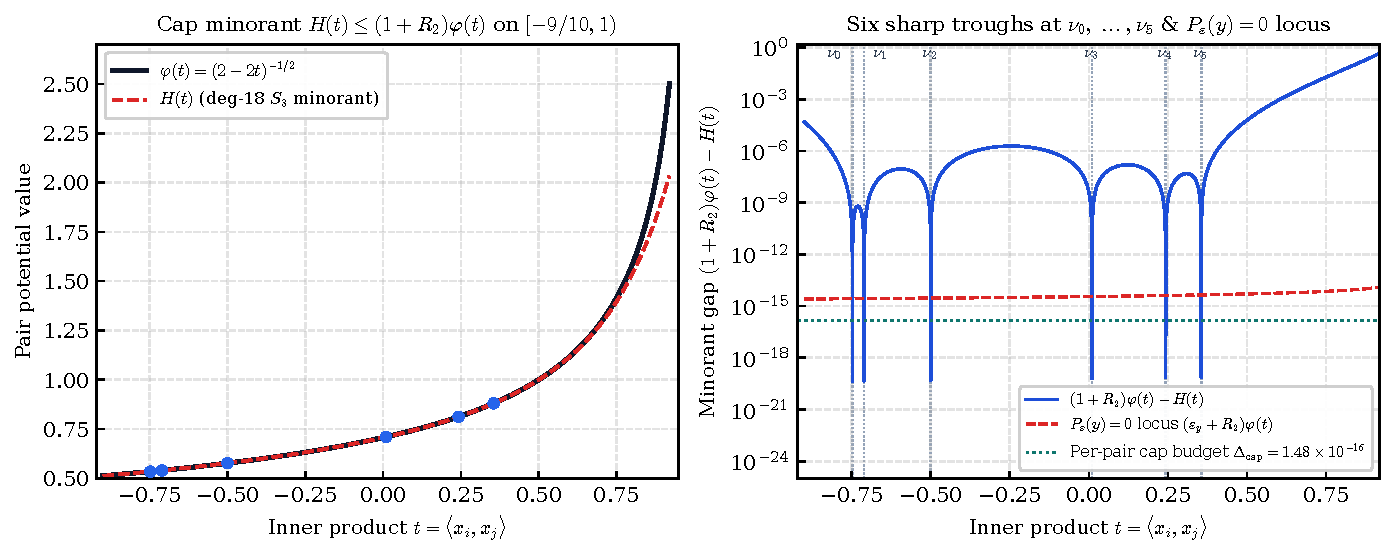
\includegraphics[width=0.98\textwidth]{figures/fig_minorant.pdf}
  \caption{Evaluated directly from the exact integer coefficients of \texttt{H\_int} in \texttt{CapCertHarmData.lean} ($S_2 = 2^{152}$). Left: $\varphi(t)$ vs.\ the degree-$18$ $S_3$-invariant minorant $H(t)$ on $[-9/10, 1)$, with the six TTP inner-product levels marked. Right: log-scale gap $(1+R_2)\varphi(t) - H(t)$ revealing six sharp zero-gap troughs at $\nu_0,\dots,\nu_5$, cleanly piercing both the exact $P_\varepsilon(y)=0$ locus $(\varepsilon_y + R_2)\varphi(t)$ and the per-pair cap budget $\Delta_{\mathrm{cap}} = 1.48\times 10^{-16}$.}
  \label{fig:minorant}
\end{figure}

\begin{table}[htbp]
  \centering
  \caption{The seven degree-$37$ Bernstein exclusion intervals \texttt{bp0}--\texttt{bp6} in $y = \sqrt{(1-t)/2}$ and the six windows between them, mapped to $t = 1 - 2y^2$ (rounded outward to $6$ decimal places). Each window lies within $9.2\times 10^{-5}$ of the corresponding $\nu_k(z^*)$.}
  \label{tab:bernstein}
  \small
  \renewcommand{\arraystretch}{1.15}
  \setlength{\tabcolsep}{4pt}
  \begin{tabular}{@{}cccc@{}}
    \toprule
    Piece & Excluded $y \in [a_\ell, b_\ell]$ & Next window & Window in $t = 1-2y^2$ \\
    \midrule
    \texttt{bp0} & $[0,\, 56773/100000]$           & Tube $5$ ($\nu_5$) & $[0.355183,\, 0.355366]$ \\
    \texttt{bp1} & $[56781/100000,\, 15383/25000]$ & Tube $4$ ($\nu_4$) & $[0.242590,\, 0.242763]$ \\
    \texttt{bp2} & $[61539/100000,\, 35181/50000]$ & Tube $3$ ($\nu_3$) & $[0.009668,\, 0.009838]$ \\
    \texttt{bp3} & $[2199/3125,\, 433/500]$        & Tube $2$ ($\nu_2$) & $[-0.500086,\, -0.499912]$ \\
    \texttt{bp4} & $[17321/20000,\, 92479/100000]$ & Tube $1$ ($\nu_1$) & $[-0.710622,\, -0.710473]$ \\
    \texttt{bp5} & $[92483/100000,\, 46737/50000]$ & Tube $0$ ($\nu_0$) & $[-0.747628,\, -0.747477]$ \\
    \texttt{bp6} & $[46739/50000,\, 9747/10000]$   & ---                & ($t \in [-0.900080, -0.747628]$ excluded) \\
    \bottomrule
  \end{tabular}
\end{table}

\section{Combinatorial Rigidity and Procrustes Ball Entry}\label{sec:rigidity}

\subsection{Certified Gram-determinant masks and $28$-leaf DFS rigidity}\label{subsec:l4-dfs}
From \texttt{CapCert.cap\_tube\_forcing}, every off-diagonal Gram entry $t_{ij}$ ($i \ne j$) lies within $\rho = 10^{-4}$ of some $\nu_k(z)$.
Since the minimum spacing between distinct $\nu_a(z), \nu_b(z)$ over $[z_{\mathrm{lo}}, z_{\mathrm{hi}}]$ exceeds $g_{\min} \approx 0.03701 > 2\rho$, each unordered pair $\{i,j\}$ has a \emph{unique} color $C_0(i,j) \in \{0,\dots,5\}$, and the scaled entry $10^5 t_{ij}$ lies inside an explicit integer interval \texttt{nodeIv}$(C_0(i,j))$ (\texttt{RigidityL4Data.lean}).

Two geometric constraints prune the $6^{36}$ possible edge colorings of $K_9$:
\begin{enumerate}[leftmargin=2.2em]
  \item \textbf{$3$-point Gram positivity:} Any three unit vectors satisfy $\det_3(a,b,c) := \det G(t_{01}, t_{02}, t_{12}) \ge 0$. Scaled integer interval evaluation (\texttt{checkTriSound}, verified by \texttt{decide +kernel}) rules out every color triple whose interval upper bound is strictly negative, leaving $181$ valid ordered triples out of $216$ (packed into the $216$-bit mask \texttt{triNat}).
  \item \textbf{$4$-point linear dependence in $\R^3$:} Any four vectors in $\R^3$ are linearly dependent, so their $4\times 4$ Gram determinant vanishes identically: $\det_4(t_{01}, t_{02}, t_{03}, t_{12}, t_{13}, t_{23}) = 0$ (\texttt{StageB.det4\_eq\_zero\_of\_unit} in \texttt{ThreePoint.lean}, line~105). Scaled integer interval evaluation (\texttt{checkK4Sound}, verified by \texttt{decide +kernel}) rules out every $6$-tuple of $K_4$ edge colors whose $\det_4$ interval excludes $0$ (i.e.\ strictly positive or strictly negative), leaving only $552$ valid ordered $K_4$ colorings out of $46{,}656$ (packed into \texttt{k4Nat}).
\end{enumerate}

To break $S_9$ symmetry without loss of generality, sort vertices $1,\dots,8$ so that $C(0,1) \le C(0,2) \le \dots \le C(0,8)$.
A recursive bit-encoded depth-first search \texttt{checkAll} assigns edges of $K_9$ incrementally, pruning at every edge via \texttt{triMask} and \texttt{k4Mask} and requiring every complete coloring that survives to belong to a precomputed list \texttt{leafWitnesses} of just $28$ complete $K_9$ colorings.
Two kernel checks prove:
\begin{itemize}[leftmargin=2em]
  \item \texttt{l4\_k9\_complete : checkAll 46 1 0 0 = true} (exhaustive completeness: every valid sorted coloring hits one of the $28$ leaves);
  \item \texttt{leaves\_iso\_ok : leafWitnesses.all checkWitness = true} (each of the $28$ leaves carries an explicit permutation $\tau \in S_9$ mapping its edge colors verbatim onto the canonical TTP pattern \texttt{nodeOfN}).
\end{itemize}
Soundness of the bit-encoded DFS against the geometric invariants (\texttt{RigidityL4.lean}) therefore guarantees a permutation $\sigma \in S_9$ such that
\begin{equation}\label{eq:gram-window}
  \bigl|\ip{x_{\sigma(i)}}{x_{\sigma(j)}} - \ip{\TTP(z)_i}{\TTP(z)_j}\bigr| \;\le\; \frac{1}{10000}
  \qquad \text{for all } i \ne j.
\end{equation}
(In our independent Stage~A check at $\rho = 10^{-6}$, full unsampled $K_9$ enumeration without symmetry breaking recovers exactly $30{,}240 = 9!/12$ labeled survivors---matching the exact $S_9$ orbit of $\TTP(z^*)$, whose automorphism group is $D_{3h} \cong D_3 \times C_2$ of order $12$.)

\subsection{Quantitative Procrustes bound into the $1/500$ Frobenius ball}\label{subsec:l5-procrustes}
Write $X = \TTP(z) \in \R^{9\times 3}$ and $Y = P_\sigma \mathrm{toMat}(x) \in \R^{9\times 3}$.
By~\eqref{eq:gram-window}, the Gram matrix difference $\Delta G = Y Y^\top - X X^\top$ has zero diagonal and off-diagonal entries bounded by $10^{-4}$, so $\Frob{\Delta G} \le \sqrt{72}\cdot 10^{-4} \le \texttt{sqrt72Up}\cdot 10^{-4}$.
For $z \in [z_{\mathrm{lo}}, z_{\mathrm{hi}}]$, the $3\times 3$ scatter matrix $S(z) = X^\top X = \mathrm{diag}(\frac{9}{2}-3z^2,\, \frac{9}{2}-3z^2,\, 6z^2)$ is strictly well-conditioned with certified spectral bounds $\lambda_3(S) \ge l_3 = 1485363/500000 \approx 2.970726$ and $\lambda_1(S) \le u_1 = 1507319/500000 \approx 3.014638$.
Applying the pre-existing formal polar-factorization / Procrustes chain \texttt{TableB5Chain.chain\_convert\_A} (built over \texttt{TableB5Core}, \texttt{TableB5Trace}, \texttt{TableB5Polar}, and \texttt{TableB5Uncond}) produces an orthogonal matrix $Q \in O(3)$ satisfying
\[
  \Frob{X - YQ} \;\le\; \left(\frac{\sqrt{u_1}\,u_1}{l_3^2} + \frac{2\sqrt{2}}{\sqrt{l_3}}\right)\Frob{\Delta G}
  \;\le\; C_{A,\mathrm{hi}} \cdot 10^{-4} \;\le\; \frac{1}{500},
\]
where $C_{A,\mathrm{hi}} \approx 18.957127$ (\texttt{RigidityL4.rigidity\_to\_ball}, line~790).
Finally, \texttt{LocalMinL6.iso\_of\_orthogonal} (line~2022) converts $Q \in O(3)$ into a Lean linear isometry $g_1 : \R^3 \simeq_{\mathrm{li}} \R^3$ such that $y_i := g_1(x_{\sigma(i)})$ satisfies
\begin{equation}\label{eq:frob-ball}
  \sum_{i=0}^8 \norm{y_i - \TTP(z^*)_i}^2 \;=\; \Frob{X - YQ}^2 \;\le\; \left(\frac{1}{500}\right)^2.
\end{equation}

\section{Strict Local Minimality and Global Uniqueness}\label{sec:local}

Let $P := \TTP(z^*)$ where $z^* \in [z^*_{\mathrm{lo}}, z^*_{\mathrm{hi}}]$ satisfies $\mathrm{critGap}(z^*) = 0$, and let $y \in \mathrm{SphereConfig}\;9$ satisfy~\eqref{eq:frob-ball}.
Our goal is to prove \texttt{LocalMinL6.local\_min\_ball} (line~1780):
\begin{equation}\label{eq:local-min-goal}
  E(P) \;\le\; E(y), \qquad \text{and } E(y) = E(P) \implies \exists\, g \in O(3),\;\forall i,\; y_i = g(P_i).
\end{equation}

\subsection{Compact $O(3)$ rotational gauge fixing}\label{subsec:gauge}
Consider the continuous functional $A \mapsto \sum_{i=0}^8 \ip{P_i}{A y_i}$ on the compact set $\{A \in \mathcal{L}(\R^3) : \forall v, \norm{Av} = \norm{v}\} \cong O(3)$.
Let $g \in O(3)$ be a global maximizer (\texttt{LocalMinL6.exists\_gauge}, line~627), and set $y'_i := g(y_i)$ and $d_i := y'_i - P_i$.
Comparing $g$ with the identity gives
\[
  \sum_{i=0}^8 \norm{d_i}^2 \;\le\; \sum_{i=0}^8 \norm{y_i - P_i}^2 \;\le\; \left(\frac{1}{500}\right)^2,
\]
and first-order optimality along every rational Cayley rotation in the $(a,b)$-plane yields the exact rotational orthogonality conditions
\begin{equation}\label{eq:rot-gauge}
  \sum_{i=0}^8 \bigl(P_{i,a} d_{i,b} - P_{i,b} d_{i,a}\bigr) \;=\; 0 \qquad \forall\, a,b \in \{0,1,2\}.
\end{equation}
Since $\norm{y'_i} = \norm{P_i} = 1$, we also have the exact radial identity $\ip{P_i}{d_i} = -\frac{1}{2}\norm{d_i}^2$.

\subsection{Exact criticality and algebraic Bregman--Young bound}\label{subsec:bregman}
Let $\lambda_P(z^*)$ (for the $6$ prism vertices) and $\lambda_C(z^*)$ (for the $3$ caps) be the radial Lagrange multipliers
\[
  \lambda_P(z^*) := \sum_{j \ne 0} \varphi(\ip{P_0}{P_j})^3 \ip{P_0}{P_j}, \qquad
  \lambda_C(z^*) := \sum_{j \ne 6} \varphi(\ip{P_6}{P_j})^3 \ip{P_6}{P_j}
\]
(closed forms \texttt{lamP}, \texttt{lamC}).
Direct evaluation using $\mathrm{critGap}(z^*) = 0$ verifies the exact equilibrium identity (\texttt{LocalMinL6.ttp\_critical}, line~378)
\begin{equation}\label{eq:critical}
  \sum_{j \ne i} \varphi(\ip{P_i}{P_j})^3 P_j \;=\; \lambda_{\mathrm{orb}(i)}(z^*)\, P_i \qquad \forall\, i \in \{0,\dots,8\}.
\end{equation}
For each pair $i < j$, write $\tau_{ij} := \ip{y'_i}{y'_j} - \ip{P_i}{P_j} = L_{ij} + q_{ij}$, where $L_{ij} := \ip{P_i}{d_j} + \ip{d_i}{P_j}$ and $q_{ij} := \ip{d_i}{d_j}$.
Because $\norm{d_i} \le 1/500$, we have $|\tau_{ij}| \le 1/200$ and $\ip{P_i}{P_j} + 1/200 < 1/2$.
For $\varphi(t) = (2-2t)^{-1/2}$ we have $\varphi'(t) = \varphi(t)^3$ and $\varphi''(t) = 3\varphi(t)^5$, and $\varphi''$ is increasing on $(-\infty, 1)$. A mean-value argument (\texttt{LocalMinL6.breg\_ge\_quad}, line~490) gives, for all $\tau_{\max} \ge 0$, $|\tau| \le \tau_{\max}$ and $t_0 + \tau_{\max} < 1$,
\[
  \varphi(t_0 + \tau) - \varphi(t_0) - \varphi(t_0)^3 \tau
  \;\ge\; \frac{3}{2}\,\varphi(t_0 - \tau_{\max})^5\, \tau^2.
\]
We apply this with $t_0 = \nu_k(z^*)$ and $\tau_{\max} = 1/200$, and write $a_k := \frac{99}{100}\cdot\frac{3}{2}\varphi(\nu_k(z^*) - \frac{1}{200})^5$ (\texttt{ac5Val}). Young's inequality in the form $(L+q)^2 \ge \frac{99}{100}L^2 - 100\, q^2$, the bound $\frac{3}{2}\varphi(\nu_k - \frac{1}{200})^5 \le 1$ for every $k$ (\texttt{c5\_le\_one\_ok}), and $q_{ij}^2 \le \norm{d_i}^2 \norm{d_j}^2 \le \frac{1}{2}(1/500)^2(\norm{d_i}^2 + \norm{d_j}^2)$ separate the quadratic part from the higher-order remainder.
Summing over all $36$ pairs and substituting~\eqref{eq:critical} and $\ip{P_i}{d_i} = -\frac{1}{2}\norm{d_i}^2$ yields
\begin{equation}\label{eq:E-ge-Qpen}
  E(y') - E(P) \;\ge\; Q_{\mathrm{pen}}(z^*, d) - 10\sum_{i=0}^8 \ip{P_i}{d_i}^2 - 400\left(\frac{1}{500}\right)^2 \sum_{i=0}^8 \norm{d_i}^2,
\end{equation}
where the $27$-variable quadratic form (\texttt{LocalMinL6.Q\_pen}) is
\begin{multline*}
  Q_{\mathrm{pen}}(z, d) = -\frac{1}{2}\sum_i \lambda_{\mathrm{orb}(i)}\norm{d_i}^2 + \sum_{i<j}\varphi(\nu_{ij})^3\ip{d_i}{d_j} + \sum_{i<j} a_{k(i,j)} L_{ij}^2 \\
  + 10\sum_i \ip{P_i}{d_i}^2 + 5\sum_{a<b}\Bigl(\sum_i (P_{i,a}d_{i,b} - P_{i,b}d_{i,a})\Bigr)^2,
\end{multline*}
whose last (rotational) term vanishes by~\eqref{eq:rot-gauge}.

\subsection{Integer-Cholesky Hessian lower bound and coercivity}\label{subsec:hessian}
Writing $v \in \R^{27}$ for the flattened displacement vector of $d$, so that $Q_{\mathrm{pen}}(z, d) = v^\top H_{\mathrm{true}}(z) v$, the module \texttt{LocalMinL6Data.lean} stores a rational matrix $H_{\mathrm{rat}}$ and an integer matrix $C_{27}$ (both at scale $10^6$) and checks by \texttt{decide +kernel}: (i) \texttt{H\_iv\_ok}: scaled integer interval arithmetic on $[z^*_{\mathrm{lo}}, z^*_{\mathrm{hi}}]$ places every entry of $H_{\mathrm{true}}(z)$ within $5\times 10^{-5}$ of $H_{\mathrm{rat}}$; (ii) \texttt{H\_chol\_ok}: every entry of $10^{-12}C_{27}C_{27}^\top$ is within $10^{-5}$ of $H_{\mathrm{rat}} - \frac{1}{25} I$. Hence every entry of $E := H_{\mathrm{true}}(z) - \frac{1}{25}I - 10^{-12}C_{27}C_{27}^\top$ satisfies $|E_{pq}| \le 6\times 10^{-5}$, and by Cauchy--Schwarz $|v^\top E v| \le 6\times 10^{-5}\bigl(\sum_p |v_p|\bigr)^2 \le 27\cdot 6\times 10^{-5}\,\norm{v}^2$.
Since $v^\top C_{27}C_{27}^\top v \ge 0$ and $\frac{1}{25} - 27\cdot 6\times 10^{-5} = 0.03838 \ge \frac{37}{1000}$, we obtain (\texttt{LocalMinL6.hessian\_lower\_bound}, line~1576)
\[
  Q_{\mathrm{pen}}(z^*, d) \;\ge\; \frac{37}{1000} \sum_{i=0}^8 \norm{d_i}^2.
\]
Finally, since $\ip{P_i}{d_i}^2 = \frac{1}{4}\norm{d_i}^4 \le \frac{1}{4}(1/500)^2\norm{d_i}^2$, combining with~\eqref{eq:E-ge-Qpen} gives
\[
  E(y) - E(P) \;=\; E(y') - E(P) \;\ge\; \left(\frac{37}{1000} - \frac{402.5}{250000}\right)\sum_{i=0}^8 \norm{d_i}^2
  \;\ge\; \frac{1}{30}\sum_{i=0}^8 \norm{d_i}^2.
\]
Hence $E(P) \le E(y)$, and if $E(y) = E(P)$ then $d_i = 0$ for all $i$, so $y_i = g^{-1}(P_i)$.
Unwinding $y_i = g_1(x_{\sigma(i)})$ yields $x_i = (g^{-1} \circ g_1^{-1})(P_{\sigma^{-1}(i)})$ with $g^{-1} \circ g_1^{-1} \in O(3)$ and $\sigma^{-1} \in S_9$, completing the proof of Theorem~\ref{thm:main}.

\section{Kernel-Checked Formalization in Lean~4}\label{sec:lean}

Nothing about the numerical SDP solvers (SDPA-GMP) or Python export scripts is trusted; they serve only to discover integer certificate data. Every mathematical claim is verified from scratch inside the Lean~4 kernel.

\subsection{Pure integer Cholesky, binary bit-tries, and $19$-slice $2\text{D}$-Kronecker evaluation}\label{subsec:kron}
Three engineering techniques make the degree-$18$ $S_3$ cap certificate checkable in the Lean~4 kernel without \texttt{native\_decide}:
\begin{enumerate}[leftmargin=2.2em]
  \item \emph{Zero-remainder integer Cholesky.} Both the harmonic blocks $F_k$ and the SOS blocks $B_r$ are stored directly as integer Cholesky factors $C C^\top$ rather than $M = LDL^\top + \Delta$, so positive semidefiniteness is automatic by \texttt{sq\_nonneg} with zero diagonal-dominance overhead; any tiny rounding mismatch is absorbed into the explicit sparse residual polynomial $\mathrm{res}$ and bounded by its $\ell^1$ coefficient norm.
  \item \emph{Binary bit-trie evaluation (\texttt{PolyKronFast.Trie}).} Evaluating a degree-$18$ trivariate polynomial identity via a single $3\text{D}$ Kronecker substitution $p(2^w, 2^{wD}, 2^{wD^2})$ would require $w D^2 \approx 240 \times 19^2 \approx 86{,}000$-bit integers inside the kernel. Instead, we prove a \emph{$2\text{D}$-Kronecker multi-slice zero theorem} (\texttt{PolyKronFast.eq\_zero\_of\_kev2\_slices}, line~559): if $f(u,v,t)$ has degrees $< D_2$ in $u$ and $v$, degree $d$ in $t$, and coefficient $\ell^1$-norm $\le L$, and $f(2^{w(T)}, 2^{w(T)D_2}, T) = 0$ for more than $d$ distinct integers $T$, each with $L \cdot \max(1,|T|)^d < 2^{w(T)}$, then $f \equiv 0$.
  For $d = 18$ and $D_2 = 19$, this replaces one $86{,}000$-bit evaluation by $19$ independent evaluations at $T \in \{-9,\dots,9\}$ with adaptive bit-widths $w(T) \in [184, 242]$ (max integer width $\approx 4{,}600$ bits), each packaged in its own Lean module \texttt{CapCertSosSlice\{M9..9\}.lean} and checked in parallel by \texttt{decide +kernel}.
  Inside each slice, basis-monomial tables are stored in a binary bit-trie \texttt{Trie $\Z$} for $O(\log N)$ lookup in kernel reduction.
  \item \emph{Zero metavar chunking.} Splitting \texttt{res\_slack\_int} ($1{,}330$ terms) into $14$ chunks prevents elaborator stack depth issues while maintaining zero \texttt{set\_option} overrides in \texttt{Solution.lean}.
\end{enumerate}

\subsection{Module architecture and verification record}\label{subsec:modules}
Table~\ref{tab:modules} lists all $45$ project modules in the dependency cone together with line counts and \texttt{decide +kernel} counts.

\begin{table}[htbp]
  \centering
  \caption{Lean~4 modules of the Thomson $N=9$ proof. The first group is \texttt{formal/lean/ThomsonN9/StageB/} ($32$ files, $1.75\,\mathrm{MB}$), written for this proof; the second group consists of \texttt{Solution.lean} and earlier project modules in the dependency cone.}
  \label{tab:modules}
  \footnotesize
  \renewcommand{\arraystretch}{1.10}
  \begin{tabular}{@{}>{\raggedright\arraybackslash}p{3.9cm}rr>{\raggedright\arraybackslash}p{7.3cm}@{}}
    \toprule
    Module & Lines & \shortstack[r]{\texttt{decide}\\\texttt{+kernel}} & Role / main theorem \\
    \midrule
    \texttt{ThreePoint} & $1{,}386$ & $0$ & $Q_k$, $\det G \ge 0$, $\det_4 = 0$, \texttt{cap\_assembly\_9}, \texttt{slab\_assembly\_9} \\
    \texttt{PolyKron} & $1{,}597$ & $0$ & \texttt{HasPolyRep3}, \texttt{eq\_zero\_of\_kev3\_zero}, \texttt{BPiece.nonneg}, Lemma~\ref{lem:3pt-pos} \\
    \texttt{PolyKronFast} & $682$ & $0$ & \texttt{Trie}, \texttt{eq\_zero\_of\_kev2\_slices} \\
    \texttt{SlabCertData} & $1{,}889$ & $15$ & $(2,7)$-typed $M=K=6$ integer Cholesky slab certificate \\
    \texttt{SlabCert} & $1{,}003$ & $0$ & \texttt{slab\_exclusion} \\
    \texttt{CapCertHarmData} & $211$ & $2$ & harmonic blocks, $H_{\mathrm{int}}$, $1\text{D}$ minorant \\
    \texttt{CapCertBernData} & $124$ & $9$ & Bernstein certificates \texttt{bp0}--\texttt{bp6} \\
    \texttt{CapCertSosData} & $1{,}458$ & $6$ & $S_3$-isotypic SOS blocks, residual, \texttt{eps\_gap\_ok} \\
    \texttt{CapCertSosSlice*} ($19$ files) & $19\times 12$ & $19$ & $2\text{D}$-Kronecker slice checks, $T \in \{-9,\dots,9\}$ \\
    \texttt{CapCert} & $782$ & $0$ & \texttt{cap\_tube\_forcing} \\
    \texttt{RigidityL4Data} & $223$ & $4$ & \texttt{triNat}, \texttt{k4Nat}, $28$ leaf witnesses, \texttt{l4\_k9\_complete} \\
    \texttt{RigidityL4} & $933$ & $0$ & \texttt{rigidity\_to\_ball} \\
    \texttt{LocalMinL6Data} & $309$ & $2$ & $z^*$ interval, square-root envelopes, $H_{\mathrm{rat}}$, $C_{27}$ \\
    \texttt{LocalMinL6} & $2{,}055$ & $0$ & \texttt{exists\_z\_star}, \texttt{exists\_gauge}, \texttt{local\_min\_ball} \\
    \midrule
    \texttt{Solution} & $818$ & $0$ & four challenge theorems + \texttt{thomson\_nine\_main} \\
    \texttt{TableB5*}, \texttt{TableB1*}, \texttt{TableA}, \texttt{M1Data} ($12$ files) & $6{,}629$ & $0$ & Procrustes chain \texttt{chain\_convert\_A}; M1 data \\
    \midrule
    \textbf{Total} ($45$ modules) & $\mathbf{20{,}327}$ & $\mathbf{57}$ & no \texttt{sorry}, no \texttt{native\_decide} \\
    \bottomrule
  \end{tabular}
\end{table}

Running \texttt{bash formal/lean/scripts/check.sh} executes all six automated verification steps (exiting non-zero on any failure):
\begin{enumerate}[leftmargin=2.2em,itemsep=1pt,topsep=3pt]
  \item \emph{File-identity pin:} checks the SHA-256 of all $75$ tracked files in \texttt{formal/lean/} against \texttt{SHA256SUMS.txt} (including \texttt{ComparatorChallenges/ThomsonN9.lean}) and rejects unpinned files.
  \item \emph{Full-cone token scan:} enforces zero forbidden tokens in \texttt{Solution.lean} and scans every module in \texttt{ThomsonN9/} (with comments stripped) and \texttt{lakefile.toml}, allowing only \texttt{maxHeartbeats}, \texttt{maxRecDepth}, and linter \texttt{set\_option} switches in supporting modules.
  \item \emph{Toolchain \& cache + full build:} fetches the pinned Mathlib cache (\texttt{lake exe cache get}) and runs \texttt{lake build ThomsonN9 ComparatorChallenges} ($8{,}972$ jobs), enforcing $4$ expected \texttt{sorry} warnings in \texttt{ComparatorChallenges/ThomsonN9.lean} and $0$ in \texttt{ThomsonN9/Solution.lean}.
  \item \emph{Strict axiom whitelist:} runs \texttt{scripts/CheckAxioms.lean} on all four challenge theorems, \texttt{thomson\_nine\_main}, and both admissibility lemmas, rejecting any axiom outside \texttt{\{propext, Classical.choice, Quot.sound\}}.
  \item \emph{Statement fidelity:} \texttt{scripts/compare\_statements.py} (\texttt{SKIP = set()}) compares all $36$ constants of \texttt{ComparatorChallenges/ThomsonN9.lean} against \texttt{ThomsonN9/Solution.lean} under \texttt{pp.all} + \texttt{pp.universes}, requiring \texttt{STATEMENT COMPARISON: OK} (digest \texttt{bafcdc5e\ldots 4ab735c9}).
\end{enumerate}
In addition, \texttt{bash formal/lean/scripts/negative-control.sh} runs two automated negative controls: (a) flipping the inequality of \texttt{thomson\_nine} in a scratch challenge copy and confirming \texttt{compare\_statements.py} rejects \texttt{Solution.tsv} naming only \texttt{ThomsonN9.thomson\_nine}; and (b) asserting a false certificate boolean via \texttt{decide +kernel} and confirming kernel rejection.

\section{Independent Stage~A Verification and Discussion}\label{sec:discussion}

\subsection{Independent $50$-digit Stage~A certificate chain}\label{subsec:stage-a}
Prior to formalization, we independently verified the complete proof in exact Python \texttt{Fraction} arithmetic and $50$-digit \texttt{mpmath.iv} interval arithmetic (\texttt{numerics/bounds/stage\_a\_closure.py}), certifying $z^*$ to $40$ digits, verifying all $24$ rational $LDL^\top$ blocks of the $128$-bit $M=10, K=10$ cap certificate (\texttt{certificates/n9-stage-a-r24-symcap-m090\_M10K10.json}) plus $5$ slab certificates out of process in $181\,\mathrm{s}$, performing $50$-digit $1\text{D}$ coercivity at $\rho = 10^{-6}$ ($11.35\times$ margin over $\varepsilon_{\mathrm{forcing}} \le 9.96 \times 10^{-20}$), recovering all $30{,}240$ labeled $K_9$ survivors, and certifying a $4\text{th}$-order geodesic-Procrustes Taylor local minimality radius $r^* = 0.06500$ ($\lambda_{\min}(H_0) \ge 0.1439348$, $4{,}369\times$ above the Procrustes bound). This chain is independent evidence only; the Lean proof does not rely on it.

\subsection{Outlook}\label{subsec:outlook}
With $N = 7$~\cite{ValsN72026}, $N = 8$~\cite{KLT2026,TZ2026}, and now $N = 9$ formally proved in Lean~4, the smallest open cases of the Thomson problem are $N = 10$ (conjectured $D_{4d}$ gyroelongated square bipyramid) and $N = 11$ (conjectured $C_{2v}$ configuration with four vertex orbits and no one-parameter closed family).
Two ingredients introduced here---pure-rational $S_3$-isotypic three-point SDP reduction with uncapped azimuthal harmonics $K = M$, and parallel multi-slice $2\text{D}$-Kronecker verification via binary bit-tries in the Lean~4 kernel---scale directly to higher-degree certificates needed for $N = 10$ and beyond.

\subsection*{Limitations of the verification}
All checks above use the reference Lean~4 kernel. Unlike the $N=7$ package~\cite{ValsN72026}, we have not yet run the Lean Comparator or an independent second kernel (e.g.\ \texttt{lean4export} with \texttt{nanoda}) on this development; doing so is planned for the public release. The statement comparison of Section~\ref{subsec:modules} plays the role of the Comparator for statement fidelity.

\subsection*{Use of AI tools}
Large language model--based coding and theorem-proving agents were used under the author's direction to assist with exploring and implementing the semidefinite programming reductions, generating exact integer/rational certificates, writing and debugging the Lean~4 formalization, preparing figures and exposition, and performing automated verification audits of the codebase and manuscript. The author directed the proof campaign, reviewed the repository and text, and takes full responsibility for the content. No mathematical claim relies on trusting any AI output: every theorem, certificate identity, and search argument is mechanically checked from scratch inside the Lean~4 kernel as documented in Section~\ref{sec:lean}.

\subsection*{Code and data availability}
The Lean~4 formalization, exact integer/rational certificates, Python certificate generators, and one-command verification scripts are available at \url{https://github.com/Refrain-Xe/Thomson_N-9_Campaign_Scheduling} (Lean~\texttt{v4.34.1}, Mathlib~\texttt{d13f23b7}).

\begin{thebibliography}{16}

\bibitem{Andreev1996}
N.~N. Andreev,
\emph{An extremal property of the icosahedron},
East J. Approx. \textbf{2} (1996), no.~4, 459--462.

\bibitem{BachocVallentin2008}
C.~Bachoc and F.~Vallentin,
\emph{New upper bounds for kissing numbers from semidefinite programming},
J. Amer. Math. Soc. \textbf{21} (2008), no.~3, 909--924.

\bibitem{CohnKumar2007}
H.~Cohn and A.~Kumar,
\emph{Universally optimal distribution of points on spheres},
J. Amer. Math. Soc. \textbf{20} (2007), no.~1, 99--148.

\bibitem{CohnWoo2012}
H.~Cohn and J.~Woo,
\emph{Three-point bounds for energy minimization},
J. Amer. Math. Soc. \textbf{25} (2012), no.~4, 929--958,
\href{https://arxiv.org/abs/1103.0485}{arXiv:1103.0485}.

\bibitem{deMouraUllrich2021}
L.~de~Moura and S.~Ullrich,
\emph{The Lean~4 theorem prover and programming language},
in Automated Deduction---CADE~28, Lecture Notes in Comput. Sci. \textbf{12699},
Springer, 2021, pp.~625--635.

\bibitem{ErberHockney1991}
T.~Erber and G.~M. Hockney,
\emph{Equilibrium configurations of $N$ equal charges on a sphere},
J. Phys. A \textbf{24} (1991), no.~23, L1369--L1377.

\bibitem{KolushovYudin1997}
A.~V. Kolushov and V.~A. Yudin,
\emph{Extremal dispositions of points on the sphere},
Anal. Math. \textbf{23} (1997), no.~1, 25--34.

\bibitem{KLT2026}
L.~Kryvonos, L.~Liehr, and M.~A. Taylor,
\emph{Energy minimization for eight points on the sphere},
\href{https://arxiv.org/abs/2609.22077}{arXiv:2609.22077} (2026).

\bibitem{Mathlib2020}
The mathlib Community,
\emph{The Lean mathematical library},
in Proceedings of the 9th ACM SIGPLAN International Conference on Certified Programs and Proofs (CPP~2020),
ACM, 2020, pp.~367--381.

\bibitem{Schwartz2013}
R.~E. Schwartz,
\emph{The five-electron case of Thomson's problem},
Exp. Math. \textbf{22} (2013), no.~2, 157--186.

\bibitem{Schwartz2023}
R.~E. Schwartz,
\emph{Divide and conquer: A distributed approach to five point energy minimization},
\href{https://arxiv.org/abs/2301.05090}{arXiv:2301.05090} (2023).

\bibitem{Thomson1904}
J.~J. Thomson,
\emph{On the structure of the atom: An investigation of the stability and periods of oscillation of a number of corpuscles arranged at equal intervals around the circumference of a circle; with application of the results to the theory of atomic structure},
Philos. Mag. (6) \textbf{7} (1904), no.~39, 237--265.

\bibitem{TZ2026}
J.~Tooby-Smith and A.~Zughaid,
\emph{Thomson-N-8-Warrant},
Lean~4 formalization, \url{https://github.com/jstoobysmith/Thomson-N-8-Warrant} (2026).

\bibitem{ValsN72026}
Vals~AI,
\emph{The pentagonal bipyramid is the unique minimiser of the Coulomb energy of seven points on the sphere: A three-point semidefinite proof with exact certificates, formalised in Lean~4},
Lean~4 proof package, \url{https://github.com/huwngtran/thomson-n7-lean} (2026).

\bibitem{WalesUlker2006}
D.~J. Wales and S.~Ulker,
\emph{Structure and dynamics of spherical crystals characterized for the Thomson problem},
Phys. Rev. B \textbf{74} (2006), 212101.

\bibitem{Yudin1992}
V.~A. Yudin,
\emph{Minimum potential energy of a point system of charges},
Discrete Math. Appl. \textbf{3} (1993), no.~1, 75--81
(Russian original: Diskret. Mat. \textbf{4} (1992), no.~2, 115--121).

\end{thebibliography}

\end{document}
